\noindent \textit{\textcolor{red!60!black}{
Minor Comment 1.\\
It would be helpful if the authors explored the equity payout results in a bit more detail. I would encourage the authors to try a number of different definitions including the \% change in payouts, dividend yield, \% of profits paid out as dividends, and break out changes coming from cash dividends vs. share repurchases and intensive vs. extensive margins (not paying out at all vs. paying out only somewhat).
}}

\bigskip

\noindent Using the extended dataset, we now report year-by-year results separately for total equity payout, cash dividends, and net repurchases (Table 4). The findings indicate that the effects are primarily driven by cash dividends rather than repurchases. 

In Panel A of Internet Appendix Table IA.15, we report cash dividend results conditioning on whether firms paid positive or zero dividends in the prior year (Columns 1–2), and in 1932, just before the leverage uncertainty period (Columns 3–4). The results indicate that the dividend increase is concentrated among firms that were already paying dividends: columns 1 and 3 show strong and statistically significant effects for prior payers, while columns 2 and 4 show no significant effect for non-payers. This pattern is consistent with the well-documented stickiness of dividend policy.

We also followed your suggestion and experimented with alternative dividend measures (dividend growth, dividends relative to book equity, market equity, and net income) in Panel B of Internet Appendix Table IA.15. The results are generally consistent across these specifications, with positive but not always statistically significant point estimates. In particular, because many firms report negative net income, the sample in which dividends represent a positive share of profits is relatively small.

\noindent \textit{\textcolor{red!60!black}{
Minor Comment 2.\\
It would be useful to see the coefficient on d in Table 4 column 1 of Panels A and B.
}}

\bigskip

\noindent This coefficient is now reported in all specifications.

\noindent \textit{\textcolor{red!60!black}{
Minor Comment 3.\\
What are the number of clusters in these regressions?
}}

\bigskip

\noindent With the extended sample period (1926--1940), we now cluster standard errors by both firm and year in all specifications—whether using year indicators or grouped period indicators (Before and After). This yields 543 firm clusters, corresponding to the number of unique firms in the sample, and 15 year clusters. We have added this information in the footnotes of the relevant tables.


\noindent \textit{\textcolor{red!60!black}{
Minor Comment 4.\\
What do the results look like using just the d>0 indicator variable that matches more closely to what is done in Figure 1?
}}

\bigskip

\noindent This result is now reported in Column 1 of Internet Appendix Table IA.16.

\noindent \textit{\textcolor{red!60!black}{
Minor Comment 5.\\
What are the correlations (and statistical significance) between d and co-variates in 1931--1932 period?
}}

\bigskip

\noindent We report the correlations between $d$ and other firm characteristics in the Internet Appendix Table IA.8. Because our new sample starts in 1926 rather than 1931, we report the correlations both for the 1926--1932 period as well as 1932 (hence, right before the leverage uncertainty period). As suggested by the significant differences between the $d = 0$ and $d > 0$ samples in Table 1, all correlations are statistically significant except only one for the 1932 sample. 

\noindent \textit{\textcolor{red!60!black}{
Minor Comment 6.\\
How do the authors reconcile Figure 1 and results from the rest of the paper? Figure 1 shows as the authors note that "[w]e find that leverage risk led public firms to delay investment in fixed capital for two years." That would suggest that not only does the period in 1933-1934 have a lower net investment rate than 1931-1932, but that 1935-1936 has a higher net investment rate than 1931-1932 and enough higher that the cumulative effects are 0 over this whole period. In other words, no investment is lost, just delayed. By contrast, Table 2 and 4 both suggest that 1935-1936 net investment is going to be basically identical to that in 1931-1932. That would suggest there is a cumulative effect as 1935-1936 net investment does not offset the decline in 1933-1934. It would be helpful for the authors to explicitly test 1935-1936 relative to 1931-1932 and provide some discussion for reader about which findings (the table or figure) seem most relevant and what the delay vs loss means in terms of the theories being tested (ex. Mello and Parsons 1992 would seem to suggest a delay). One natural prediction would seem to be that the reduction in uncertainty in 1935-1936 should lead to the same net investment difference as would occur in 1931-1932, plus some additional positive net investment for those treated firms. The current evidence in the main paper/tables doesn't seem to support that conclusion. 
}}

\bigskip

\noindent Thank you for this comment. You are correct that our earlier evidence was more consistent with a return to usual investment levels rather than a delay. Our revised empirical design, where we report the coefficient on $d$ interacted with year indicators, makes this clearer. Table 3 and Figure 3 of the revised manuscript report net investment results from 1926 to 1940, with $d$ interacted with year indicators. Using 1932 as the omitted category, we find that higher $d$ predicts lower investment only in 1933 and 1934. Column 2 of Table 3 shows some evidence of a statistically significant recovery for exposed firms in 1935. After 1935, investment differentials across $d$ converge back to pre-1933 levels. We now briefly note this finding in Section 5.2 (third paragraph).

\noindent \textit{\textcolor{red!60!black}{
Minor Comment 7.\\
If the gold clauses hurt firm value, how come we don't see that in Tobin's Q? It would be helpful to show explicitly that the equity value of these firms are hurt by the risk during this period or if the authors find it isn't provide a plausible explanation for why.
}}

\bigskip 

\noindent Thank you for this observation. As clarified in Section 5.1, our conceptual framework emphasizes that debt overhang creates a wedge between marginal and average $Q$. Accordingly, investment should be lower for firms with more severe debt overhang, even after controlling for average $Q$—which is precisely what we find in the data.

That said, you are right that we might also expect a larger decline in average $Q$ in 1933 and 1934 for firms with higher gold clause exposure, but we do not find this. In Table \ref{tab:Q}, we regress $Q$ on $d$ interacted with four indicators—1926–1932 (Before), 1933, 1934, and 1935–1940 (After)—with Before as the omitted category. If anything, high-$d$ firms experienced a slightly smaller decline in average $Q$ in 1933. When we add controls interacted with year, as in Column 2 of Table 6, the coefficient for 1933 becomes negative but remains relatively small.

 \begin{table}[h]
    \centering
    \begin{tabular}{lcc}
    \toprule
   & Without controls & With controls \\
    \midrule
  1933 $\times d$ &0.18$^{**}$ & -0.06$^{*}$\\
                  &(0.06)      &(0.03) \\
  1934 $\times d$ & 0.01 & -0.02\\
                & (0.08) & (0.04)\\
  After $\times d$ & 0.02 & 0.03\\
                   &(0.10) & 0.05\\
    \bottomrule
    \end{tabular}
    \caption{\\ Average $Q$}
    \label{tab:Q}
    \end{table}


\noindent 

The return evidence reported in our previous response suggests that the equity value of the gold-exposed firms was indeed affected by the uncertainty of leverage generated by the abrogation. When we narrow down our analysis of equity value to important events related to the enforceability of the gold clause---such as when Congress passed the Joint Resolution in June 1933 and when the Supreme Court rendered its decision---we find that the returns (raw and abnormal) on gold-exposed firms were significantly larger than those of the overall market.

Identifying why average $Q$ was unaffected in 1933 and 1934 is admittedly difficult. However, if we interpret average $Q$ as a measure of investment opportunities, the absence of a differential effect on $Q$ suggests that the abrogation did not differentially impact the investment opportunities of exposed firms. Rather, the investment decline we document reflects the reduced incentive of exposed firms to invest due to debt overhang: even in the presence of similar investment opportunities, equityholders of exposed firms had weaker incentives to fund new projects because a larger share of the returns would accrue to bondholders in the event of default.

\bigskip

\noindent \textit{\textcolor{red!60!black}{
Minor Comment 8.\\
How should we reconcile the findings in this paper with those in Figure 4 of Edwards et al. (2015)? They find no effect of gold clauses until 1934, while this paper finds evidence in 1933. They find no reduction in the risks of the gold clause in 1935, while this paper suggests there are. It would be good to include a detailed discussion of these divergent assumptions/findings and why the authors don't believe they are problematic. At its surface high frequency data on prices for otherwise virtually identical bonds with and without gold clauses trading on the same days seems like a fairly clean approach to examine the pricing effects of gold clauses, so it seems important to reconcile with those findings.
}}

\bigskip

\noindent Thank you for raising this point. To address it, we carefully reread \cite{Edwards2015} to better understand the source of the difference in our results. We have identified several possibilities. Before expanding on them, we begin with a brief summary of \cite{Edwards2015}'s results.

In their paper, \cite{Edwards2015} study how the abrogation of the gold clause has affected the Treasury's borrowing cost. To do so, they compare the yields of a portfolio of bonds that were issued before the abrogation of the gold clause (which included the gold clause) to the yield of bonds that were issued after the abrogation of the gold clause (which did not include the gold clause). Because the bonds in these two groups have different effective durations, the portfolios are dynamically rebalanced daily over their sample to match the effective duration. For convenience, we report the time series of the yield spread reported in Figure 4 of their article in Figure \ref{fig:R1_gold_yield_spread} below. In this figure, the y-axis is the yield difference between bonds without a gold clause and bonds with a gold clause,
\begin{align*}
    y = \text{portfolio yield}_{\text{Without Gold}} - \text{portfolio yield}_{\text{With Gold}}.
\end{align*}
\begin{figure}[h]
  \centering
  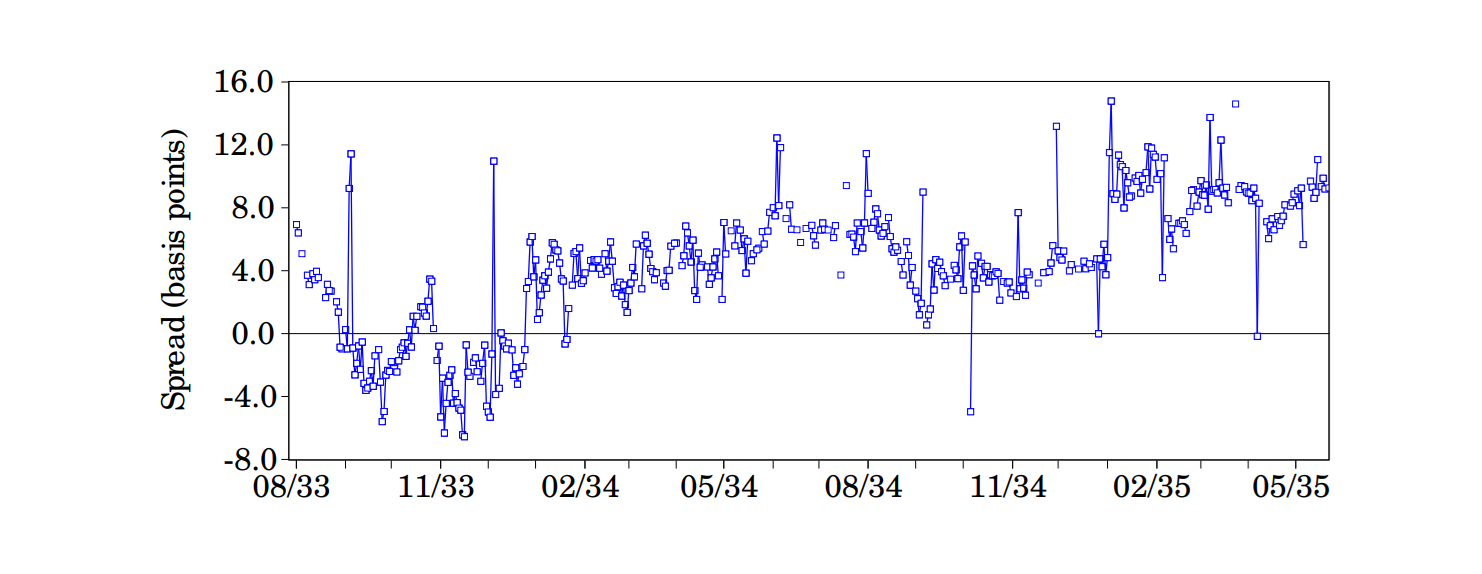
\includegraphics[width=\linewidth]{../../referee-responses-figures/r1-gold-yield-spread.png}
  \caption{Yield spread between gold and non-gold denominated bonds}
  \label{fig:R1_gold_yield_spread}
\end{figure}

\noindent A positive value of y indicates a lower yield on gold bonds, which in turn corresponds to a price premium on bonds with a gold clause.

As noted in your comment (as well as by \cite{Edwards2015} themselves), a striking feature of this plot is the absence of any reduction in the gold premium following the Supreme Court's February 1935 decision to uphold the abrogation of the gold clause. In fact, the spread appears to widen in the aftermath of the Court's decision, a puzzling observation for which we propose two potential explanations.

The first explanation requires additional historical context regarding the Supreme Court's ruling on the abrogation's constitutionality. The Court's decision upholding the abrogation applied to both private and public contracts, but the justices employed distinct legal reasoning for each. For private contracts, the Court ruled 5-4 that the abrogation was constitutional. However, for public contracts, the Court ruled 8-1 that the abrogation was \textit{un}constitutional. Ironically, despite ruling the abrogation unconstitutional, the Court determined that the plaintiffs had not suffered recoverable damages and therefore awarded no compensation.

It seems plausible that US Treasury bondholders interpreted the decision as leaving the door open for future favorable rulings should public bond holders succeed in proving damages. Supporting this interpretation, \cite{Edwards2015} notes that in the years following the Court's decision, additional lawsuits challenging the constitutionality of the abrogation were filed, though the Supreme Court declined to hear these cases. For convenience, we reproduce the relevant passage from \cite{Edwards2015} below:

``Curiously, the premium for gold clause bonds persisted even after the Supreme Court decision. One possible interpretation of this result is that investors continued to believe that a return to the gold standard might occur once macroeconomic fundamentals improved. Another possible interpretation is that the market believed there was some probability that the Supreme Court would reverse itself and grant some compensation to holders of gold clause securities. Indeed, during the years to come, a number of lawsuits regarding the abrogation made it through the court system. The Supreme Court, however, refused to hear any of these cases.''

To provide additional detail on the legal differences between private and public contract cases, we have added a footnote to the ``Historical background'' section. This footnote reads ``The Court heard four cases: two concerning private contracts and two concerning public contracts. For private contracts, the Court ruled 5-4 that the abrogation was constitutional. For public contracts, the Court ruled 8-1 that the abrogation was \textit{un}constitutional. However, despite finding the abrogation of gold clauses in public contracts unconstitutional, the Court determined that the plaintiffs had not suffered recoverable damages and thus awarded no compensation.'' We abstain from providing a detailed discussion of the subtlety of the Supreme Court's ruling in that section to keep the focus on the background information most relevant to our aim.

Before expanding on the second set of factors that might explain the difference between our results and those of \cite{Edwards2015}, we should note that the yield comparison exercise performed in their paper is deceptively challenging. Extracting the market value of the gold clause by comparing the yield of two dynamically managed portfolios of Treasury bonds is difficult since US Treasury bonds in the 1930s were highly bespoke securities (see \cite{Lehner2025} for a comprehensive treatment of the measurement challenges involved in constructing historical Treasury yield spreads). We expand below on the idiosyncratic attributes of US Treasuries during this period, emphasizing how these features may create yield differentials between the two bond types that are unrelated to the gold clause.

First, as \cite{Edwards2015} note in their paper, 9 out of 10 bonds in their sample were callable. Moreover, as they also indicate, most call options for the gold-denominated bonds were deep in the money. In contrast, the non-gold denominated bonds had just been issued and their call options were likely out of the money. This implies that changes in yields over their sample period might reflect changes in call option values in addition to changes in the value of the gold clause.

Second, the US Treasury was issuing bonds with various tax statuses: some bonds were fully taxable, some were partially taxable, and some were nontaxable. This raises the possibility that the difference between gold and non-gold denominated bonds reflects differences in tax treatment rather than gold clause valuation. \cite{Edwards2015} do not address this issue in the most recent version of the paper I have access to.

Third, the US Treasury was also issuing so-called "flower bonds." These bonds were redeemable at par value upon the holder's death and provided estate tax benefits. This raises the possibility that differences between gold and non-gold denominated bonds reflect the varying prevalence of flower bonds in the sample considered by \cite{Edwards2015}. This issue is also left unaddressed in their analysis.

To summarize, we believe that differences in the legal context of the abrogation between public and private gold clauses may explain part of the discrepancy between our results and those of \cite{Edwards2015}. Moreover, the yield comparison exercise performed in their paper is potentially affected by measurement issues. These issues remain unaddressed in the most recent version of \cite{Edwards2015} available to us, which complicates interpretation of the evidence presented above.

Thank you again for your constructive and insightful comments. The new analyses, guided by your suggestions, have significantly strengthened the empirical evidence and enhanced our understanding of the mechanism, providing a more comprehensive perspective on this period.
